
\section{Ejercicio 3}

\subsection{Desarrollo}

Para poder resolver el problema de TaskBatch lo que hacemos es generar cant$\_$bloqueos valores aleatorios no repetidos que no estén ubicados fuera de total$\_$cpu. Usando la
función rand y en cada momento guardarnos el resultado en un vector. Siempre revisamos los valores hasta el que estamos agregando para asegurarnos de que no estamos repitiendo
ninguno. Lo generado por esto podría no estar ordenado, así que le hacemos un sort al resultado. Por último ciclaremos total$\_$cpu veces y en las posiciones donde se tendría que 
bloquear(que estén en el vector que nos armamos) hacemos la llamada usa$\_$IO con duración de 1. Si caemos en el caso donde no se debe hacer ninguna llamada bloqueante, 
entonces simplemente ejecutamos usa$\_$CPU con total$\_$cpu de tiempo.

\subsection{Experimentación}

Siguiendo lo pedido por enunciado, realizaremos el gráfico del loteEj3.tsk usando el FCFS y nos queda lo siguiente:

Lote:

TaskBatch 20 10  //Bloqueo 10 veces en una tarea de 20 ciclos de duración

TaskBatch 10 6 	//Bloqueo 6 veces en una tarea de 10 ciclos de duración

TaskBatch 34 14 //Bloqueo 14 veces en una tarea de 34 ciclos de duración

\begin{figure}[H]
  \centering
    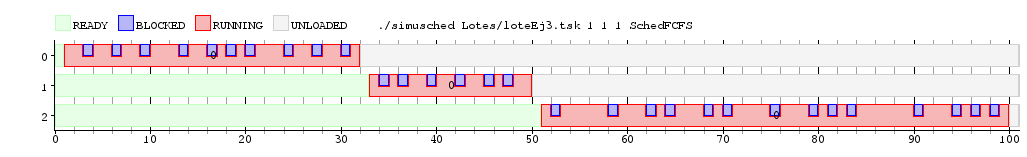
\includegraphics[width=1.1\textwidth]{imagenes/Ej3Experimento1.png}
  \caption{loteEj3.tsk con FCFS con un core}
\end{figure}

Podemos ver que la primer tarea ejecuta 10 llamadas bloqueantes y que cada una tiene duración de 1 ciclo. Pasa lo mismo con la segunda y la tercera que se ejecutan durante 10
 y 34 ciclos respectivamente con 6 y 14 llamadas bloqueantes.

\begin{figure}[H]
  \centering
    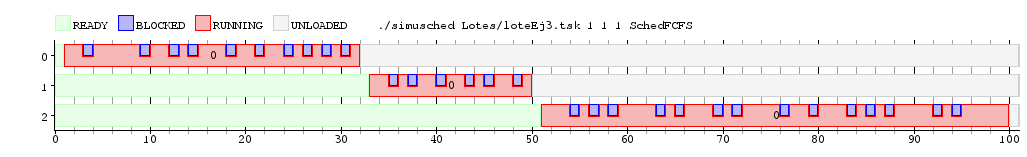
\includegraphics[width=1.1\textwidth]{imagenes/Ej3Experimento2.png}
  \caption{loteEj3.tsk con FCFS con dos cores}
\end{figure}

Para poder asegurar la aleatoriedad del TaskBatch ejecutamos nuevamente con el mismo lote de tareas y observamos que las llamadas bloqueante aperecen en momentos diferentes.